\documentclass[11pt,a4paper]{article}

\usepackage[T1]{fontenc}
\usepackage[margin=1cm]{geometry}
\usepackage{pgf-umlcd}

\usepackage{fontspec}
\setsansfont{Source Sans Pro}

\title{\textbf{UML}}
\author{Class Diagram}
\date{Book Store Management}

\begin{document}

\maketitle

\sffamily

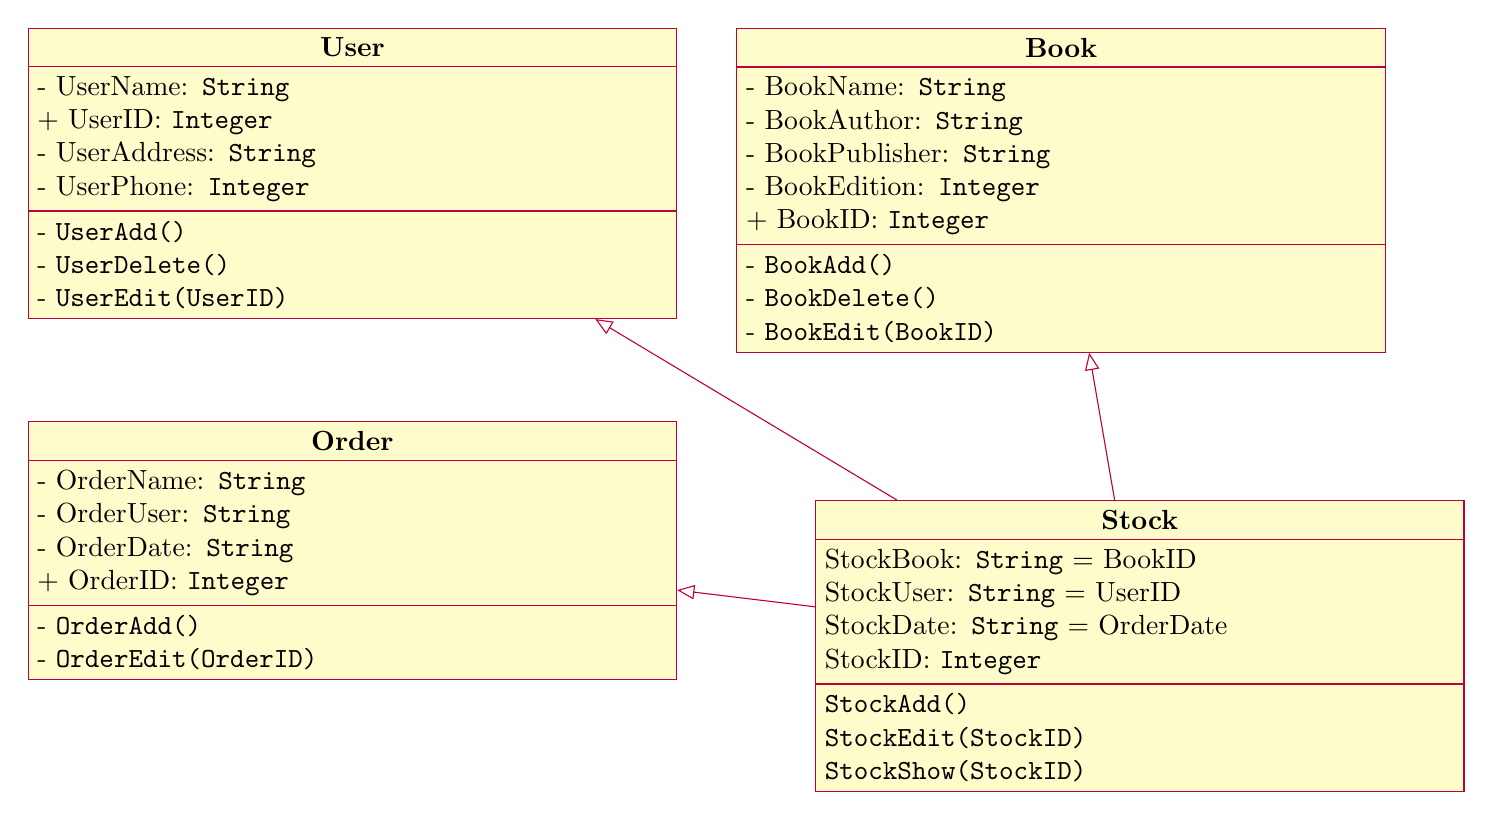
\begin{tikzpicture}
	\begin{class}[text width=8cm]{User}{0,0}
		\attribute{- UserName: \texttt{String}}
		\attribute{+ UserID: \texttt{Integer}}
		\attribute{- UserAddress: \texttt{String}}
		\attribute{- UserPhone: \texttt{Integer}}
		\operation{- \texttt{UserAdd()}}
		\operation{- \texttt{UserDelete()}}
		\operation{- \texttt{UserEdit(UserID)}}
		% \operation[0]{name(parameters list): type of value returned}
	\end{class}

	\begin{class}[text width=8cm]{Book}{09,0}
		\attribute{- BookName: \texttt{String}}
		\attribute{- BookAuthor: \texttt{String}}
		\attribute{- BookPublisher: \texttt{String}}
		\attribute{- BookEdition: \texttt{Integer}}
		\attribute{+ BookID: \texttt{Integer}}
		\operation{- \texttt{BookAdd()}}
		\operation{- \texttt{BookDelete()}}
		\operation{- \texttt{BookEdit(BookID)}}
	\end{class}

	\begin{class}[text width=8cm]{Order}{00,-05}
		\attribute{- OrderName: \texttt{String}}
		\attribute{- OrderUser: \texttt{String}}
		\attribute{- OrderDate: \texttt{String}}
		\attribute{+ OrderID: \texttt{Integer}}
		\operation{- \texttt{OrderAdd()}}
		\operation{- \texttt{OrderEdit(OrderID)}}
	\end{class}

	\begin{class}[text width=8cm]{Stock}{10,-06}
		\inherit{User}
		\inherit{Book}
		\inherit{Order}
		\attribute{StockBook: \texttt{String} = BookID}
		\attribute{StockUser: \texttt{String} = UserID}
		\attribute{StockDate: \texttt{String} = OrderDate}
		\attribute{StockID: \texttt{Integer}}
		\operation{\texttt{StockAdd()}}
		\operation{\texttt{StockEdit(StockID)}}
		\operation{\texttt{StockShow(StockID)}}
	\end{class}
\end{tikzpicture}

\end{document}
